\documentclass{minimal}
\usepackage[paperwidth=353.04pt,paperheight=456pt,margin=0pt,noheadfoot]{geometry}
\usepackage{graphicx,tikz}
\pagestyle{empty}
\begin{document}
\begin{tikzpicture}[remember picture,overlay,x=1pt,y=1pt]
\begin{scope}[shift={(current page.south west)}]
  \node[anchor=south west,inner sep=0] at (0,0)
    {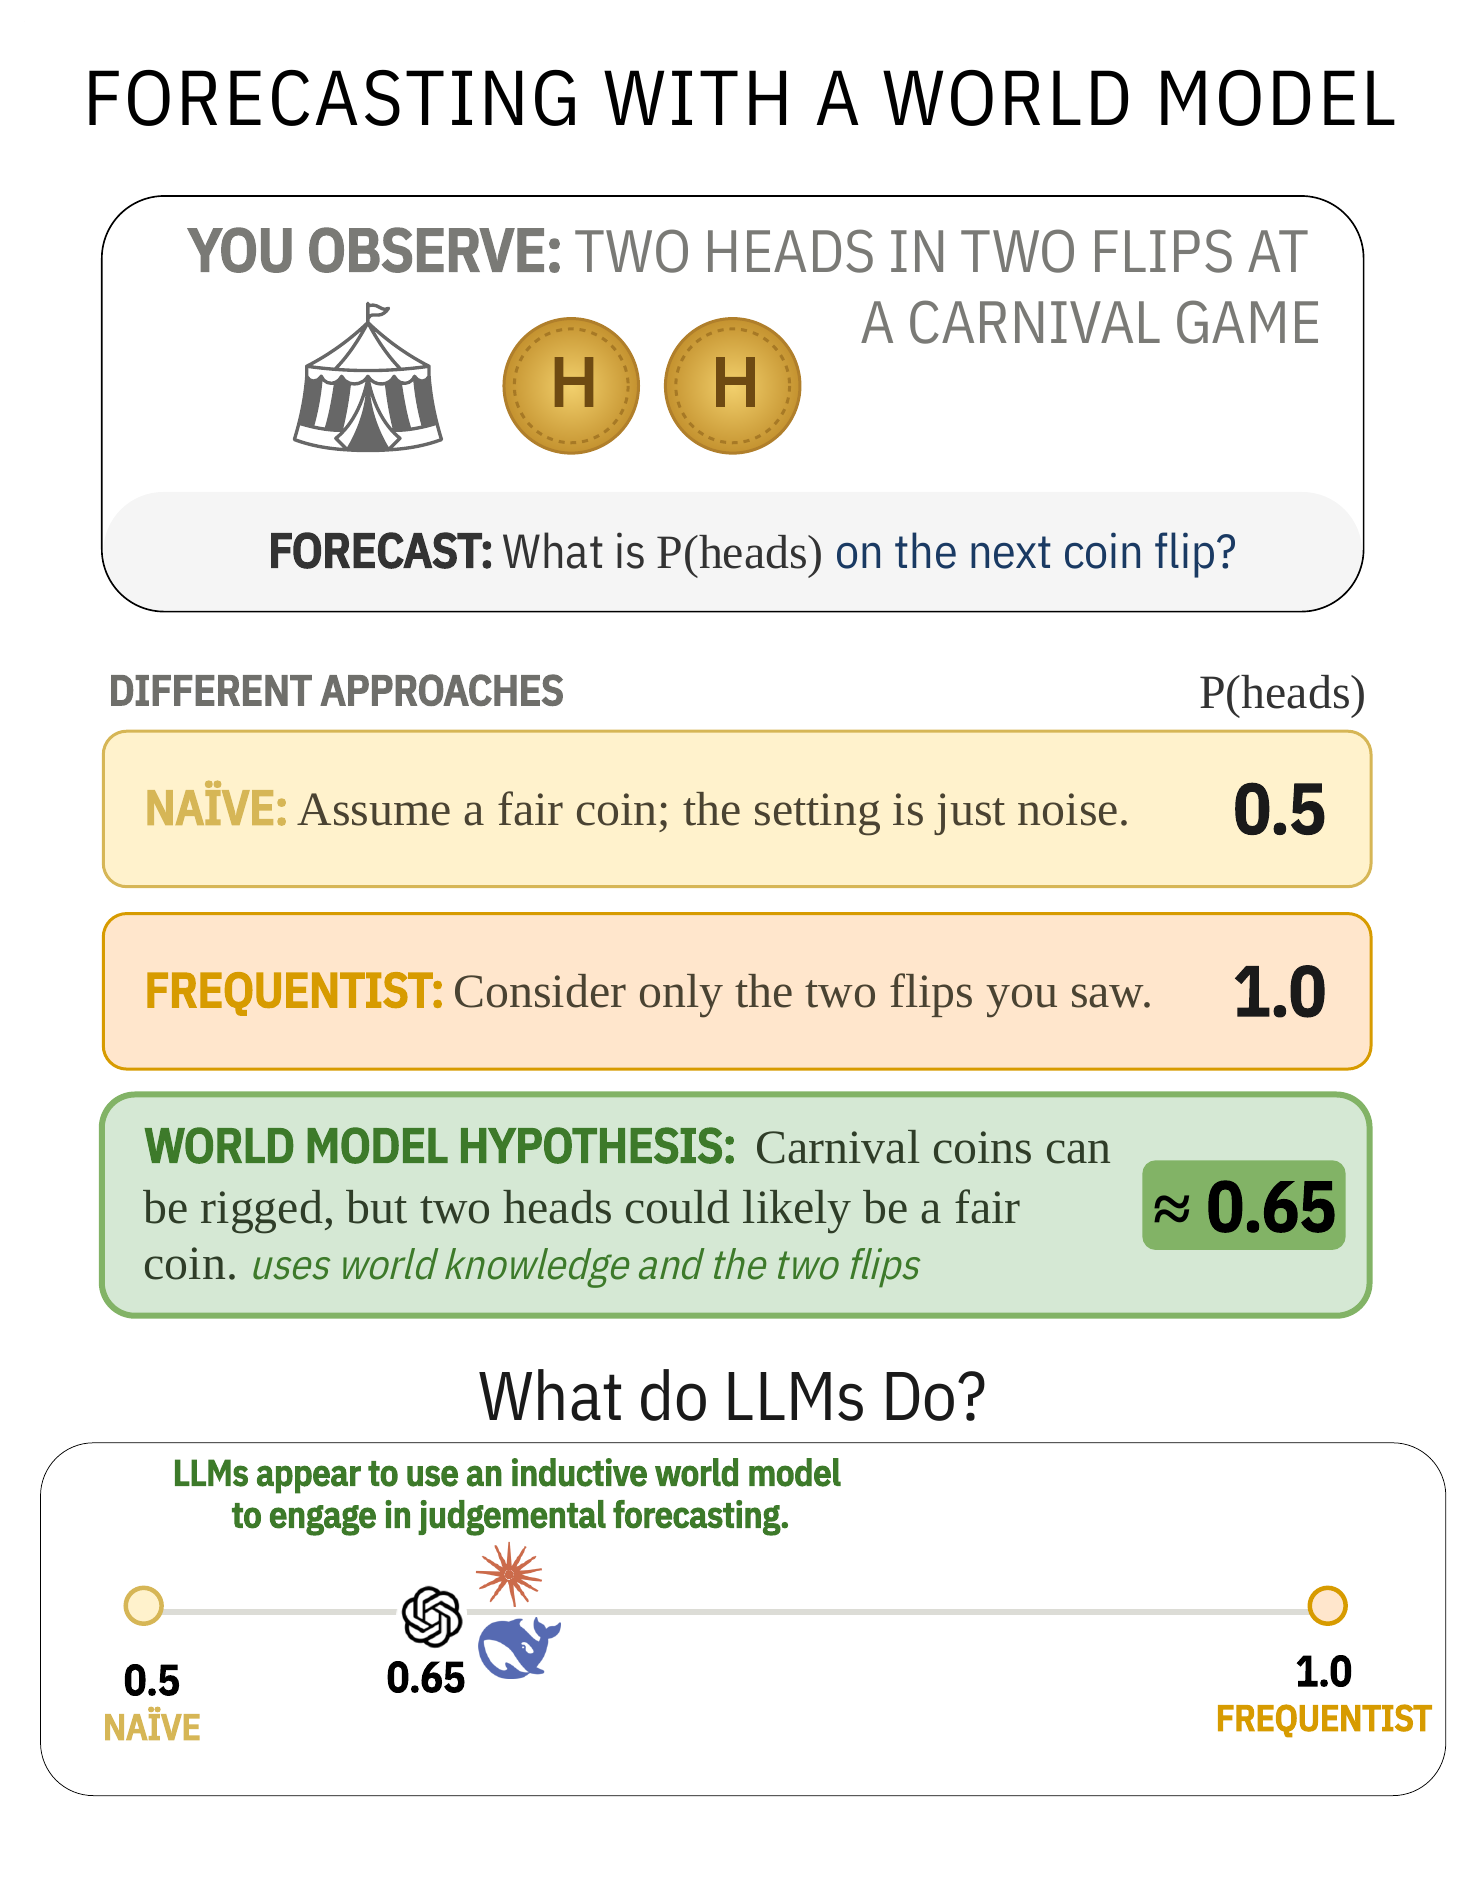
\includegraphics[width=353.04pt]{teaser_base.png}};

  % Change only the original bold category label. The replacement is rendered
  % in the original IBM Plex Sans Condensed Medium at the original 16 px size.
  \definecolor{teaserGreen}{HTML}{D5E8D4}
  \fill[teaserGreen] (33,172.5) rectangle (180.5,190);
  \node[anchor=south west,inner sep=0] at (34.48,173.66)
    {
\includegraphics{teaser_label.pdf}};

  % The three displayed model means average to .679, which rounds to .68.
  % Preserve the original approximation sign and replace the numeric labels.
  \definecolor{teaserGreenDark}{HTML}{82B366}
  \fill[teaserGreenDark] (287.8,156) rectangle (320.7,178);
  \node[anchor=south west,inner sep=0] at (289.285,147.54)
    {
\includegraphics{teaser_value_big.pdf}};
  \fill[white] (91.8,46.5) rectangle (112.5,61);
  \node[anchor=south west,inner sep=0] at (92.1,46.5)
    {
\includegraphics{teaser_value_small.pdf}};

  % Keep the original three-model result strip, but remove the interpretive
  % heading and sentence that were added above it. Re-center the unchanged
  % logos, mean, endpoints, and labels inside the original rounded box.
  \fill[white] (0,0) rectangle (353.04,139);
  \draw[gray!65,line width=0.45pt,rounded corners=8pt]
    (24,79) rectangle (329,138);
  \node[anchor=south west,inner sep=0] at (29,84)
    {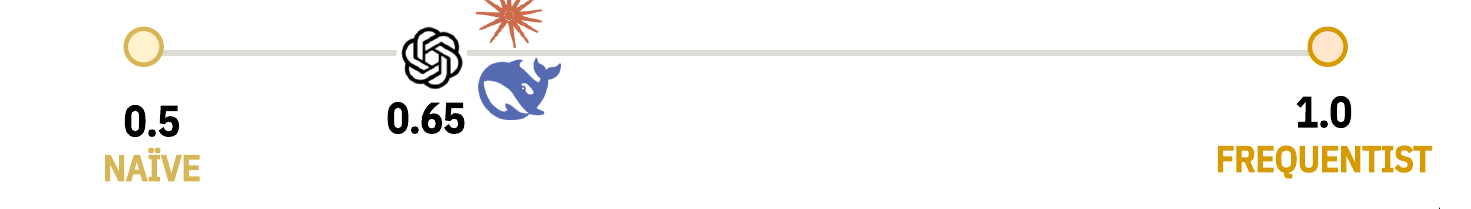
\includegraphics[width=295pt]{teaser_models_strip.png}};

  % Restore the Claude mark clipped by the original row crop.
  \begin{scope}
    \clip (124.0,115.8) rectangle (138.2,129.9);
    \node[anchor=south west,inner sep=0] at (29,57.328)
      {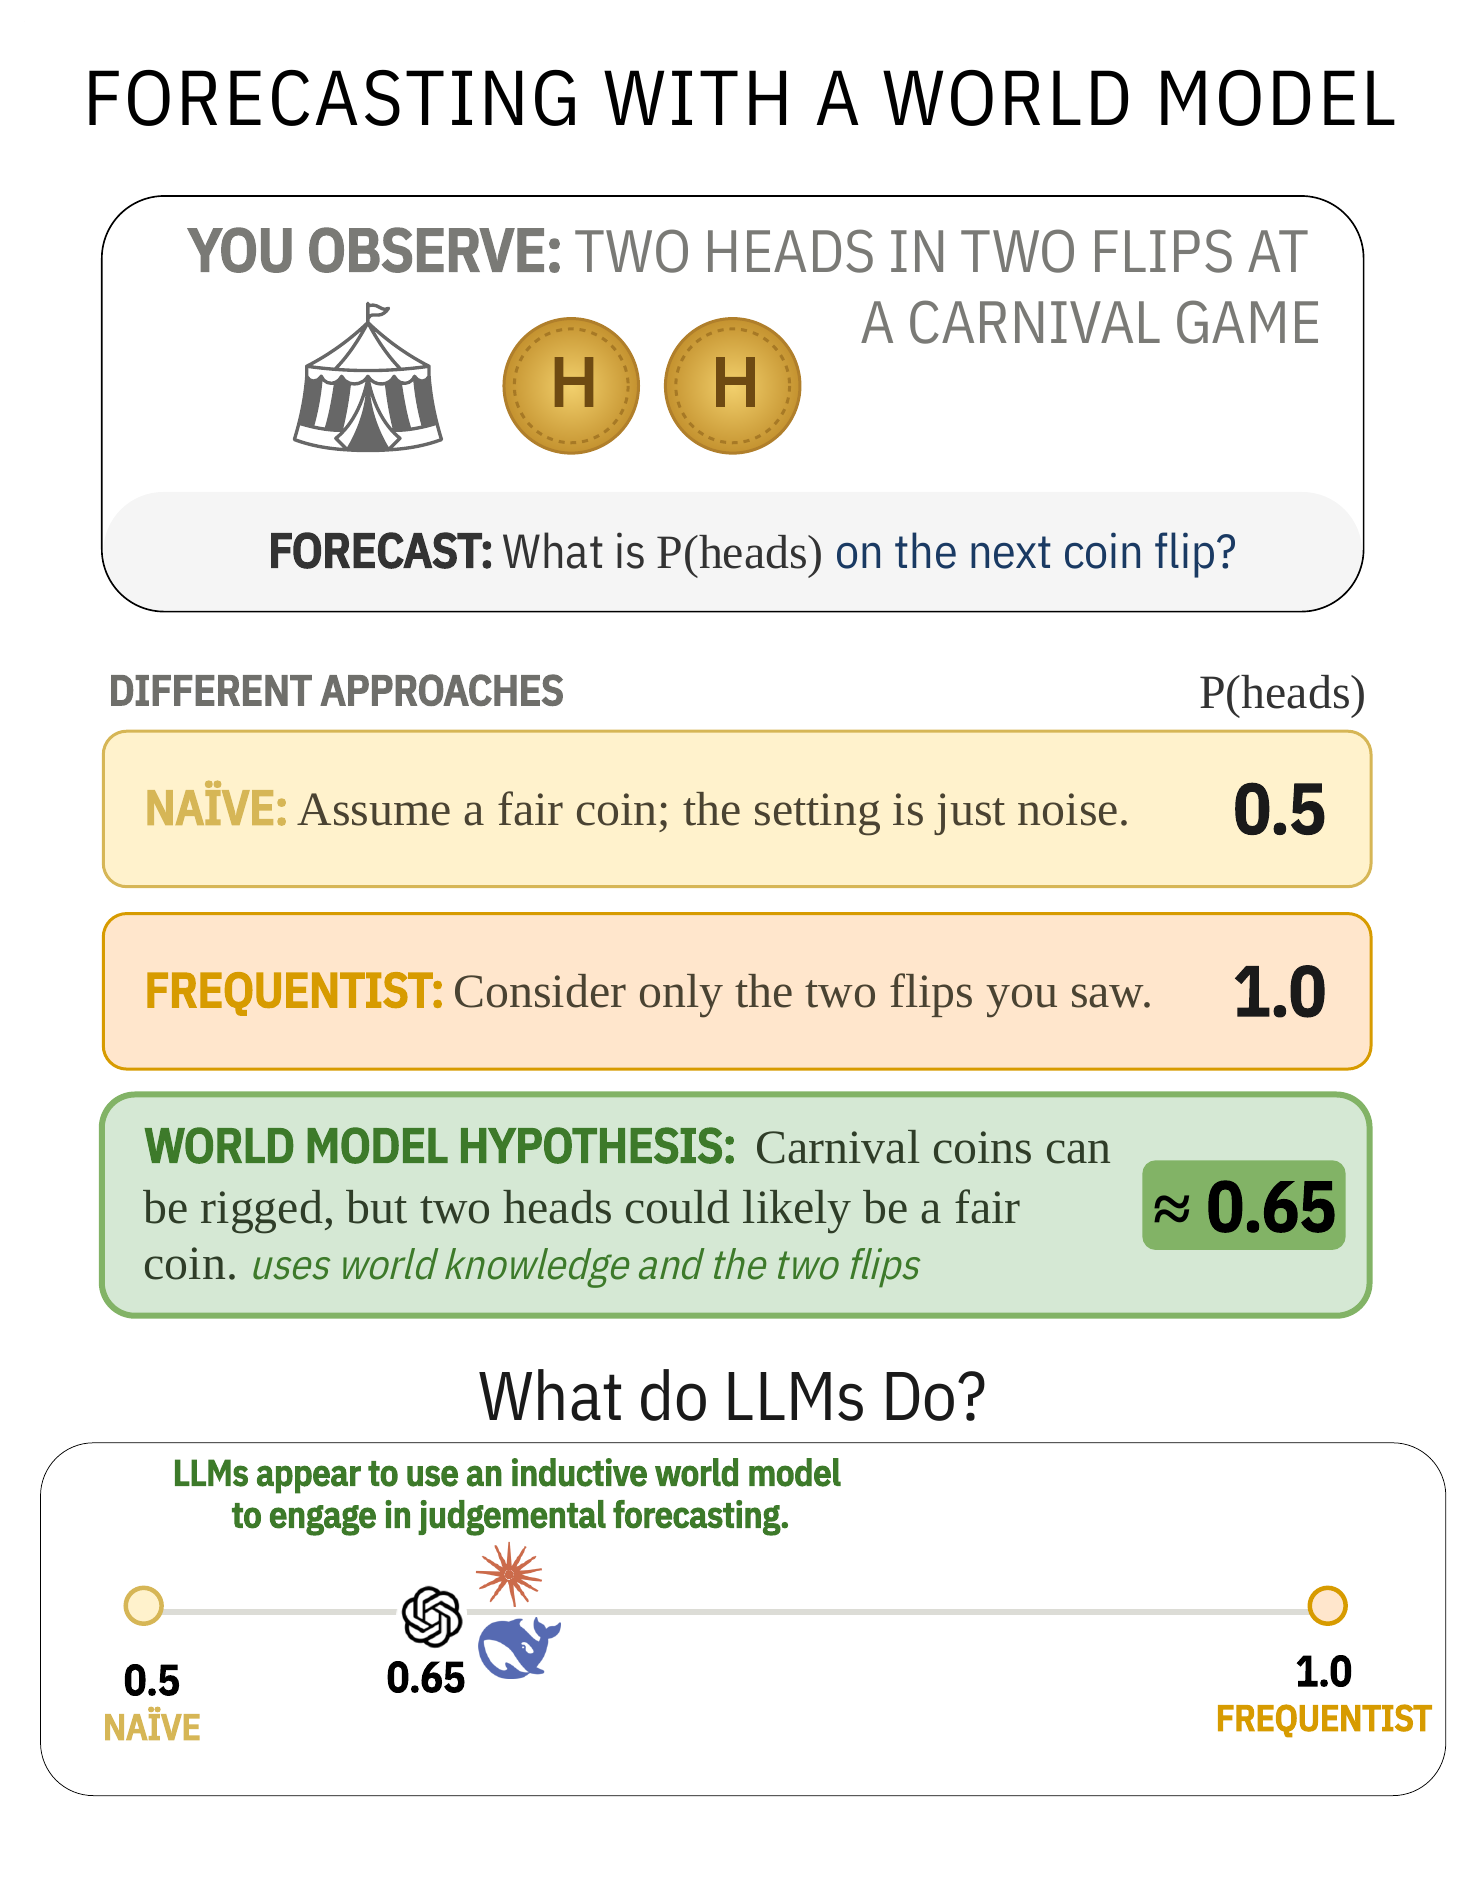
\includegraphics[width=295pt]{teaser_base.png}};
  \end{scope}
  \fill[white] (105.7,95.3) rectangle (123.1,107.5);
  \node[anchor=south west,inner sep=0] at (105.9,95.3)
    {
\includegraphics[width=20.85pt]{teaser_value_small.pdf}};
\end{scope}
\end{tikzpicture}
\null
\end{document}
